\section{Performance and Validation}

\subsection{Performance and Scaling}
We perform weak scaling tests for simulations of convection preceding ignition in a spherical, full-star sub-Chandrasekhar mass white dwarf.
The simulation setup remains the same as reported in Section 3 of \cite{MAESTRO_AMR} and originally used in \cite{MAESTRO_convection}, and thus we emphasize that these scaling tests are performed using meaningful, scientific calculations.
Here, we perform simulations using $256^3, 512^3, 768^3, 1024^3, 1280^3$, and $1536^3$ grid cells on a spatially uniform grid (no AMR).
We divide each simulation into $64^3$ grids, so this simulations contain between 64 grids ($256^3$) and 13,824 grids ($1536^3$).
These simulations were performed using the NERSC cori system on the Intel Xeon Phi (KNL) partition.
Each node contains 68 cores, each capable of supporting up to 4 hardware threads (i.e., a maximum of 272 hardware threads per node).
For these tests, we assign 4 MPI tasks to each node, and 16 OpenMP threads per MPI process.
Each MPI task is assigned to a single grid, so our tests use between 64 and 13,824 MPI processes (i.e., between 1,024 and 221,184 total OpenMP threads).
For $64^3$ grids we discovered that using more than 16 OpenMP threads did not decrease the wallclock time due to a lack of work available per grid; in principle one could use larger grids, fewer MPI processes, and more threads per MPI process to obtain a flatter weak scaling curve, however the overall wallclock time would increase except for extremely large numbers of MPI processes (beyond the range we tested here).
Thus, the more accurate measure of weak scaling is to consider the number of MPI processes, since the scaling plot would look virtually identical for larger thread counts.
Note that the largest simulation used roughly 36\% of the entire computational system.
%%%%%%%%%%%%%%%%%%%%%%%%%%%%%
\begin{figure}[htb]
\begin{center}
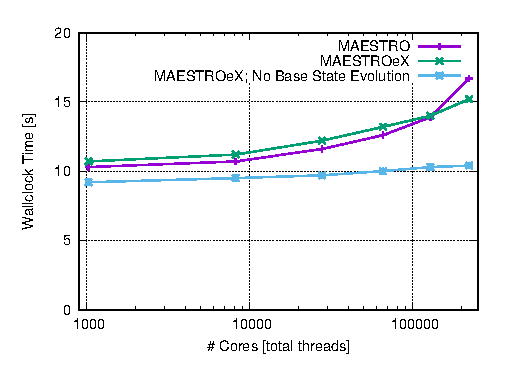
\includegraphics[width=2.75in]{./figs/MAESTRO_scaling1}
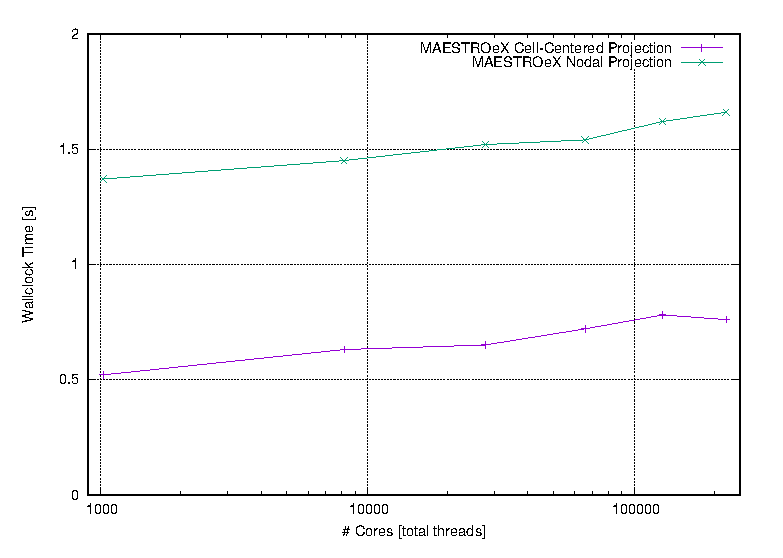
\includegraphics[width=2.75in]{./figs/MAESTRO_scaling2}
\caption{\label{fig:scaling} (Left) Weak scaling results for a spherical, full-star sub-Chandrasekhar mass white dwarf calculation using the original MAESTRO code, MAESTROeX, and MAESTROeX with base state evolution disabled.  Shown is the average wallclock time per time step.
(Right) Weak scaling results showing the average wallclock time per time step spent in the cell-centered and nodal linear solvers within a full time step of the aforementioned simulations.}
\end{center}
\end{figure}
%%%%%%%%%%%%%%%%%%%%%%%%%%%%%

In the left panel of Figure \ref{fig:scaling} we compare the wallclock time per time step as a function of total core count (in this case, the total number of OpenMP threads) for the original FBoxLib-based MAESTRO implementation to the AMReX MAESTROeX implementation.
These tests were performed using the original temporal integration strategy in \cite{MAESTRO_V}, noting that the new temporal integration scheme gives very similar performance results.\MarginPar{quantify this?... and also irregular dr case?}
We also include a plot of MAESTROeX without base state evolution.
Comparing the original and new implementations, we see similar scaling results except for the largest simulation, where MAESTROeX performs better.
We see that the increase in wallclock time from the smallest to largest simulation is roughly 42\%.
We also note that without base state evolution, the code runs 14\% faster for small problems, and scale mush better
However, for the case without base state evolution, the overall runtime is faster and the increase in wallclock time from the smallest to largest simulation is roughly 13\%.
This is quite remarkable since there are 3 linear solver per time step (2 cell-centered Poisson solves used in the MAC projection, and a nodal Poisson solve used to compute the updated cell-centered velocities).
Contrary to our prior assumptions, the linear solves are not the primary scaling bottleneck in this code.
In the right panel of Figure \ref{fig:scaling}, we isolate the wallclock time required for these linear solves and see that (i) the linear solves only use 20-23\% of the total computational time, and (ii) the increase in the solver wallclock time from the smallest to largest simulation is only 28\%.
Further profiling reveals that the primary scaling bottleneck is the average operator.
The averaging operator requires binning the sum of Cartesian data onto one-dimensional arrays holding every possible mapping radius.
This amounts to at least 24,384 points (for the $256^3$ simulation) up to 883,584 point (for the $1536^3$ simulation).
The averaging operator requires a global sum reduction over all processors, and the communication of this data is the primary scaling bottleneck.
For the simulation with base state evolution, this averaging operator is only called once per time step (as opposed to 14 times per time step when base state evolution is included).
The difference in total wallclock times with and without base state evolution is almost entirely due to the averaging.
Note that as expected, advection, reactions, and calls to the equation of state scale almost perfectly, since there is only a single parallel communication call to fill ghost cells.

\subsection{AMR Performance}
Show 3D reacting bubble rise performance.
Show 3-level spherical performance (stats won't be as good but explain why: refining a larger percentage of grid)
Images of grid configuration.

\subsection{White Dwarf Convection}
white dwarf convection runs with 3 algorithms (original, new temporal, new temporal + irregular base state)

Show 3-level wdconvect
